%------------------------------------------------------------------------------
%Description:  LaTeX Thesis Template main file
%Author:       silas.kalmbach@ilek.uni-stuttgart.de
%              benedikt.strahm@ilek.uni-stuttgart.de
%Created:      2021-03-10
%last change:  2022-07-18
%------------------------------------------------------------------------------

% ============= Einstellungen zur Arbeit =============

\documentclass[%
    paper=a4,
	bibliography=totoc,	% Literaturverzeichnis im Inhalt
	listof=totoc,		% Abb.- und Tab.verzeichnis im Inhalt
	listof=entryprefix, % Abkürzungen Abb./Tab. in den Verzeichnissen
    fontsize=11pt, 		% Schriftgröße
    twoside=off, 		% Off = PDF-Version, On = Booklet / Book (Gedrucktes Exemplar)
    headings=openright	% Einfügen von Leerseiten
]{scrbook}              % Dokumentenklasse: KOMA-Script Book

% ============= Einstellungen zum Kompilieren =============

\def\tikzextern{0} % Externes speichern von TIKZ-Grafiken zur Beschleunigung der Compilierungszeit. 0 = Nein; 1 = Ja
\def\mintedinstall{0} % Codedarstellung mit Minted. 0 = Nein; 1 = Ja; Um Minted zu nutzen muss Python und Pygments installiert sein. Alternative bei 0: listings
\def\tocstyle{0} % 0 = Klassisches Inhaltsverzeichnis, 1 = Modifiziertes Inhaltsverzeichnis
\def\autonomenclature{0} % 0 = Nomenclatur selbst schreiben (basic), 1 = Nomenclatur im Text berücksichtigen (siehe _symbols.tex) und anschließend generieren lassen

% ============= Randabstände =============

\usepackage[left= 2.5cm, right = 2cm, top=2.5cm]{geometry}

% ============= Präambel einbinden ============= 

% Variablen einbinden
% ============= Einstellungen Abmessungen Einband ============= 

% Breite des Buchrückens in mm, dies anpasse, siehe auch ReadMe
\newcommand\spineWidth{10}

% Hier muss nichts verändert werden
% DIN A4 Abmessungen
\newcommand\standardPageWidth{210}
\newcommand\standardPageHeight{297}

% Abmessungen Einband
\newcommand\bookCoverWidth{\numexpr\spineWidth + 2*\standardPageWidth\relax}
\newcommand\bookCoverHeight{\standardPageHeight}

% ============= Angaben zur Arbeit =============

% Hier den Titel der Arbeit angeben 
\newcommand{\TitelDerArbeit}{Xxxxx Xxxxx Xxxxx Xxxxx Xxxxx Xxxxx Xxxxx Xxxxx Xxxxx Xxxxx} 

% Hier die Art der Abschlussarbeit eingeben 
\newcommand{\TypDerArbeit}{Masterarbeit} 

% Nummerrierung der Arbeit (mit Betreuer zu klären)
\newcommand{\NummerDerArbeit}{XX} 

% Angabe des Monates der Abgabe als Wort
\newcommand{\EndeMonat}{Januar} 

% Angabe des Jahres der Abgabe
\newcommand{\EndeJahr}{20XX} 

% Hier den Betreuer der Arbeit angeben
\newcommand{\Betreuer}{Xxxxx Xxxxx} 

% Hier den Prüfer der Arbeit angeben 
\newcommand{\Pruefer}{Xxxxx Xxxxx} 

%Hier den Studierendenname der Arbeit angeben 
\newcommand{\StudentVorname}{Max} 
\newcommand{\StudentNachname}{Mustermann} 

% Hier den Professor1 des Instituts angeben 
\newcommand{\ProfEins}{Prof. Dr.-Ing. M.Arch. Lucio Blandini} 

% Hier den Professor2 des Instituts angeben 
\newcommand{\ProfZwei}{Prof. Dr.-Ing. Balthasar Nov\'{a}k} 

% Hier das Institut angeben
\newcommand{\Institut}{Institut f{\"u}r Leichtbau Entwerfen und Konstruieren} 

% Preambel einbinden
%------------------------------------------------------------------------------
%Description:  LaTeX Thesis Template preamble
%Author:       silas.kalmbach@ilek.uni-stuttgart.de
%Created:      2021-03-10
%------------------------------------------------------------------------------

% ============= Dokumentinformationen =============

\usepackage[ 
hidelinks
]{hyperref} 
\hypersetup{ 
	pdfauthor={\StudentVorname \StudentNachname}, 
	pdftitle={\TitelDerArbeit},
	pdfsubject={\TypDerArbeit}, 
	pdfkeywords={},
	colorlinks=true, %Einfärben statt der Box
	citecolor=blue,
	linkcolor=black,
	urlcolor=blue
%	linkbordercolor={1 1 1},
%	urlbordercolor={0 0.25 0.56},
%	citebordercolor={1 1 1},
%	menubordercolor={1 1 1},
%	filebordercolor={1 1 1},
%	citebordercolor={1 1 1}
}

% ============= Farbschema =============

\usepackage{color}      %Verwendung von Farben
\usepackage{xcolor}		%Definition eigener Farben

% Uni Stuttgart Colors
\definecolor{uniSlightblue}{RGB}{0,190,255}
\definecolor{uniSdarkblue}{RGB}{0,65,145}
\definecolor{uniSdarkgrey}{RGB}{62, 68, 76}
\definecolor{uniSgreyblue}{RGB}{125,198,234}
\definecolor{uniSgrey}{RGB}{159,153,152}

% Uni Stuttgart monochrom greyscale
\definecolor{uniSblack}{RGB}{0,0,0}
\definecolor{uniSdarkgrey}{RGB}{62,68,76}
\definecolor{uniSgrey}{RGB}{159,153,152}
\definecolor{uniSlightgrey}{RGB}{185,186,187}


% ============= Standart Packages und Einstellungen =============

\usepackage{ifluatex}
\ifluatex
	\usepackage[utf8]{luainputenc} %Schriftkodierung LuaLaTeX
\else
	\usepackage[utf8]{inputenc} %Schriftkodierung PDFLaTeX
\fi

\usepackage{fancyvrb} % Sophisticated verbatim text
\usepackage[english, ngerman]{babel} %Sprachen
\usepackage{graphicx} %Einbinden von Bildern
\usepackage{amsfonts} % zusätzliche Schriftzeichen der American Mathematical Society
\usepackage{amsmath,amssymb} % zusätzliche Schriftzeichen der American Mathematical Society
\usepackage{typearea} %Aufteilung von Rändern und Textbereich
\usepackage{nicefrac}% weitere Alternative mit mehreren Zeichen für Brüche
\usepackage{pdfpages} %Einfügen von PDFs
\usepackage{appendix} %Anhang
\usepackage{fvextra} %automatic line breaking and improved math mode
\usepackage{csquotes} %inline and display quotations
\usepackage[german, nameinlink]{cleveref} % Mehr Möglichkeiten zum referenzieren
\usepackage{gensymb} %Symbole: \degree \celsius \perthousand \ohm \micro
\tolerance = 400  % möglicher Abstand zwischen den Wörtern erhöhen
\usepackage[section]{placeins} %\FloatBarrier Verhindert das Abbildungen in nachfolgenden Kapitel rutschen
\makeatletter\AtBeginDocument{\expandafter\renewcommand\expandafter\subsection\expandafter{\expandafter\@fb@secFB\subsection}}\makeatother %FloatBarrier für Subsection
\usepackage{subcaption} % Bilder nebeneinander
\captionsetup[subfigure]{list=true, labelfont=bf, position=top}
\usepackage{wrapfig} % Bilder von TExt umgeben
\usepackage{dirtree} % Darstellen von Verzeichnisstrukturen


% ============= Programmierung (Visualisierung) =============

\if 1\mintedinstall
	\usepackage[cache=false]{minted} %Highlighting von Code, Benötigt Python und Pygments hinterlegt in den Umgebungsvariablen (pip install Pygments) ,cmd Eingabe->pdflatex -synctex=1 -interaction=nonstopmode -shell-escape %.tex
	\usemintedstyle{tango, xleftmargin=20pt, linenos, fontsize=\small, breaklines=true, tabsize=4} %borland, bw, tango, frame=leftline
\fi


\usepackage{listings}
%\lstset{
%	language=python,
%	otherkeywords={1, 2, 3, 4, 5, 6, 7, 8 ,9 , 0, -, =, +, [, ], (, ), \{, \}, :, *, !},
%}

\lstdefinestyle{UniStStyle}{
%	backgroundcolor=\color{uniSlightgrey},   
	commentstyle=\itshape\color{uniSlightblue}\lstset{columns=fullflexible},
	keywordstyle=\color{uniSdarkblue},
	numberstyle=\tiny\color{uniSlightgrey},
	stringstyle=\color{uniSgreyblue},
	basicstyle=\ttfamily\small,
	xleftmargin=20pt,
%	xrightmargin=3pt,
	breakatwhitespace=false,         
	breaklines=true,                 
	captionpos=b,                    
	keepspaces=true,                 
	numbers=left,                    
	numbersep=10pt,                  
	showspaces=false,                
	showstringspaces=false,
	showtabs=false,                  
	tabsize=4
}

\lstset{style=UniStStyle}


% ============= Tabelleneinstellungen =============

\usepackage{multirow}						% ermoeglicht mehrere Zeilen in einer Tabellenzeile
\usepackage{multicol} 						% mehre Spalten auf eine Seite

\usepackage{longtable}[=v4.13]				% alternatives Tabellenpackage inkl. longtabu und Farben
\usepackage{tabu}
\usepackage{float}							% um [H] bei float Objekten verwenden zu können
\usepackage{booktabs}						% um \toprule, \midrule und \bottomrule verwenden zu können
\usepackage{tabularx}
\usepackage{tabulary}
\usepackage{csvsimple} %Excel Improtieren als CSV 
\usepackage{siunitx} %Wissenschaftliche Angabe der Einheiten \num{number}
%für Excel to Latex Add-on
\usepackage{colortbl} %Farbige Tabellen
\usepackage{rotating} %Rotieren von Tabellen
\usepackage{bigstrut} %Für Tabellen mit Vertikalen Linien

% ============= Schriftarten =============

\ifluatex
%% ============= Lua-LaTeX =============
% Prüfen ob Datei mit Schriftart UniversforUniS vorhanden:
    \IfFileExists{./_E_ressources/fonts/UniversforUniS55Rm-Regular.ttf}{
        % Wenn ja, diese Schriftart auswählen
    	\usepackage[no-math]{fontspec} 
    	\setmainfont{UniversforUniS}[
    	Extension      = .ttf,
    	Path           = _E_ressources/fonts/,
    	UprightFont    = *55Rm-Regular,
    	ItalicFont     = *45LtObl-Rg,
    	BoldFont       = *65Bd-Regular,
    	BoldItalicFont = *45LtObl-Rg,
    	]
    	\setsansfont{UniversforUniS}[
    	Extension      = .ttf,
    	Path           = _E_ressources/fonts/,
    	UprightFont    = *55Rm-Regular,
    	ItalicFont     = *45LtObl-Rg,
    	BoldFont       = *65Bd-Regular,
    	BoldItalicFont = *45LtObl-Rg,
    	]
    	%\setmonofont{}[]
    	\addtokomafont{disposition}{\rmfamily} %Überschriften selbe Schriftart wie Text
    	\renewcommand\familydefault\sfdefault % Formeln in Sans-Serif
    	\usepackage[italic, symbolgreek]{mathastext} % Formeln in Sans-Serif
    	\renewcommand\familydefault\rmdefault % Formeln in Sans-Serif
    }{
    	\usepackage[T1]{fontenc} %Richtige Trennung von Umlauten
    	\usepackage[scale=0.87]{tgheros}
    % 	\usepackage{fourier}
    	\renewcommand\familydefault\sfdefault % alles in Sans-Serif
    	\usepackage[italic, symbolgreek]{mathastext} % Formeln in Sans-Serif
    }

\else
%% ============= PDF-LaTeX =============
	\usepackage[T1]{fontenc} %Richtige Trennung von Umlauten
	\usepackage[scale=0.87]{tgheros}
%	\usepackage{fourier}
	\renewcommand\familydefault\sfdefault % alles in Sans-Serif
	\usepackage[italic, symbolgreek]{mathastext} % Formeln in Sans-Serif
\fi



\usepackage{setspace} %Zeilenabstand
\setstretch{1.05} %Zeilenabstand

\setlength{\parindent}{0pt} %Wenn Absatzabstand, dann Einzug unnötig
\setlength{\parskip}{7pt} %Absatzabstand



% ============= Kopf- und Fußzeile =============

\usepackage[automark, headsepline, autooneside=false]{scrlayer-scrpage}

% Führe nur aus, wenn nicht article als document class festgelegt wurde (frontcover.tex)
\makeatletter
\@ifclassloaded{article}{}{     
    \automark[section]{chapter}	%Automatische Kapitelangabe in Kopfzeile
    \renewcommand*{\chaptermarkformat}{} %Kapitel ohne Kapitelnummer
}
\makeatother

\renewcommand*{\sectionmarkformat}{} %Kapitel ohne Kapitelnummer
\clearpairofpagestyles %aktuelle Einetsllungen aus Kopf- und Fußzeile löschen
\setkomafont{pageheadfoot}{\small}		%Font für Kopfzeile
\setkomafont{pagefoot}{\small}  		%Font für Fußzeile
\setkomafont{pagenumber}{\small} 	%Font für Seitennummer
\KOMAoptions{headsepline = true} %Kopzeile Linie

\lehead[]{\rightmark} %Zweiseitig
\cohead[]{}
\rohead[]{\leftmark\enskip \raisebox{0.7pt}{|}\enskip \thechapter} %Darstellung Kapitel

\lefoot[\pagemark]{\pagemark}
\lofoot[]{}
\cofoot[]{}
\rofoot[\pagemark]{\pagemark} %Seitenzahl


% ============= Literatur =============

\usepackage[									
    natbib=true,			% Naturwissenschaftlich
    backend=biber,			% Biber statt BibTex verwenden. In TexStudio einstellen!
    style=numeric,			% Stil im Verzeichnis alt. authoryear
    citestyle=numeric,	    % Stil im Fließtext
    giveninits=true,										
    doi=false,				% doi nicht mit angeben
    isbn=false,				% isbn nicht mit angeben
    sorting=none,			% Sortierung des Verzeichnis nach Autor, Titel, Jahr
    % sorting=none,			% Keine Sortierung des Verzeichnisses
]{biblatex}	

\addbibresource{_D_backmatter/literatur.bib} %Bibliographiedateien laden

\urlstyle{same}	% url Schriftart anpassen auf die des Dokuments anpassen
\usepackage{xpatch}% author in bold font in bibliography
\xpretobibmacro{author}{\mkbibbold\bgroup}{}{}
\xapptobibmacro{author}{\egroup}{}{}
\xpretobibmacro{bbx:shortauthor}{\mkbibbold\bgroup}{}{}
\xapptobibmacro{bbx:shortauthor}{\egroup}{}{}
\xpretobibmacro{bbx:editor}{\mkbibbold\bgroup}{}{}
\xapptobibmacro{bbx:editor}{\egroup}{}{}


% ============= Besondere Abkürzungen ============= 

\usepackage[figurename=Abb., % Beschriftung von Abbildung zu Abb.
tablename=Tab., % Beschriftung von Tabelle zu Tab.
labelfont=bf]{caption} %Label in Bold

% Führe nur aus, wenn nicht article als document class festgelegt wurde (frontcover.tex)
\makeatletter
\@ifclassloaded{article}{}{     
    \KOMAoptions{numbers = noenddot} % der Punkt hinter den Kapiteln etc wird entfernt: 1.1. wird zu 1.1
}
\makeatother


% ============= Daten Plotten ============= 

\usepackage{svg} 

\usepackage{tikz} %Grafiken Zeichnen
\if 0\tikzextern
	\usetikzlibrary{shapes, arrows, positioning, calc, chains, scopes}
\else
	\usepackage{shellesc} % Notwendig für LuaLaTeX
	\usetikzlibrary{shapes, arrows, positioning, calc, chains, scopes, external}
	\tikzexternalize[prefix=_E_ressources/tikz/,optimize command away=\includepdf] % activate and define tikz/ as cache folder
\fi

\usepackage{pgfplots}  %Kurven, Graphen
\usepgfplotslibrary{dateplot, fillbetween, groupplots}
\pgfkeys{/pgf/number format/.cd,fixed, use comma}
\pgfplotsset{
	compat=newest,
	every axis label/.append style={font={\rmfamily}},
}
\AtBeginEnvironment{tikzpicture}{\footnotesize} %Schriftart Tabelle \small, \footnotesize

\usepgfplotslibrary{groupplots}
\usepgfplotslibrary{dateplot}

\newlength{\figureheight} %Eigene Vatiable für Längen
\newlength{\figurewidth} %Eigene Vatiable für Längen

% ============= Abkürzungen, Glossare ============= 
\usepackage[%
	nonumberlist, 			% keine Seitenzahlen anzeigen
	toc,          			% Einträge im Inhaltsverzeichnis
	section,    			% im Inhaltsverzeichnis auf section-Ebene erscheinen
    xindy={language=german-duden,codepage=utf8}, % xindy zum Indexieren verwenden -> Perl.exe muss vorher installiert werden (https://www.activestate.com/products/perl/) Weitere Informationen unter http://tug.ctan.org/tex-archive/macros/latex/contrib/glossaries/glossariesbegin.html#x1-50011
    acronym,				% Separates Akronym-Verzeichnis
    nopostdot,				% Kein Punkt am Ende einer Beschreibung im Glossar
    automake=immediate
]{glossaries}

% Glossare & Abkürzungsverzeichnisse:
% Hier ergänzen sollten weitere Glossare erstellt werden

\newglossary[lug]{lat_upp}{lus}{luo}{Latin upper case letters}              % Big Latin Letters
\newglossary[llg]{lat_low}{lls}{llo}{Latin lower case letters}         		% Small Latin Letters
\newglossary[gug]{gre_upp}{gus}{guo}{Greek upper case letters}              % Big Greek Letters
\newglossary[glg]{gre_low}{gls}{glo}{Greek lower case letters}         		% Small Greek Letters         	
\newglossary[mog]{math_op}{mos}{moo}{Mathematical Operators}               	% Mathematical Operators

\makeglossaries

% Dateien die die Definitionen der Glossare enthalten
% Abbreviations

\newacronym{cent}{cent.}{century}
\newacronym{CFD}{CFD}{Computational Fluid Dynamics}

\newacronym{DFT}{DFT}{discrete Fourier transform}

\newacronym{FEM}{FEM}{Finite Element Method}
\newacronym{FV}{FV}{Finite Volume}

\newacronym{SVG}{SVG}{Scalable Vector Graphics}
% ------------------------
% Latin Lower Case Symbols
% ------------------------
% Dummy Symbol nicht löschen, dient der Formatierung des Abstandes zwischen Symbol und Erläuterung
\newglossaryentry{dummy_lat_low}{
	type=lat_low,
	sort=ZZZ,
	name={$~~~~~~~~~~~~~~$},
	description={$~~~~~~~$}
}
\newglossaryentry{u_i}{
	type=lat_low,
	sort=u_i,
	name={$u_{i}$},
	description={Velocity components in index notation}
}
\newglossaryentry{u_ref}{
	type=lat_low,
	sort=u_ref,
	name={$u_{ref}$},
	description={Reference velocity at $z_{ref}$}
}

% ------------------------
% Latin Upper Case Symbols
% ------------------------
% Dummy Symbol nicht löschen, dient der Formatierung des Abstandes zwischen Symbol und Erläuterung
\newglossaryentry{dummy_lat_upp}{
	type=lat_upp,
	sort=ZZZ,
	name={$~~~~~~~~~~~~~~$},
	description={$~~~~~~~$}
}
\newglossaryentry{Strouhal}{
	type=lat_upp,
	sort=St,
	name={$St$},
	description={Strouhal number}
}
\newglossaryentry{Iuu}{
	type=lat_upp,
	sort=Iuu,
	name={$I_{u_{i}u_{j}}$},
	description={Turbulence intensity}
}

% ------------------------
% Greek Upper Case Symbols
% ------------------------
% Dummy Symbol nicht löschen, dient der Formatierung des Abstandes zwischen Symbol und Erläuterung
\newglossaryentry{dummy_gre_upp}{
	type=gre_upp,
	sort=ZZZ,
	name={$~~~~~~~~~~~~~~$},
	description={$~~~~~~~$}
}
\newglossaryentry{dt}{
	type=gre_upp,
	sort=dt,
	name={$\Delta t$},
	description={Time step size}
}

% ------------------------
% Greek Lower Case Symbols
% ------------------------
% Dummy Symbol nicht löschen, dient der Formatierung des Abstandes zwischen Symbol und Erläuterung
\newglossaryentry{dummy_gre_low}{
	type=gre_low,
	sort=ZZZ,
	name={$~~~~~~~~~~~~~~$},
	description={$~~~~~~~$}
}
\newglossaryentry{kappa}{
	type=gre_low,
	sort=kappa,
	name={$\kappa$},
	description={Von-Kármán constant}
}
\newglossaryentry{rho}{
	type=gre_low,
	sort=alpha,
	name={$\rho_{u_{i}u_{j}}$},
	description={Normalized autocorrelation}
}

% ------------------------
% Mathematical Operators
% ------------------------
% Dummy Symbol nicht löschen, dient der Formatierung des Abstandes zwischen Symbol und Erläuterung
\newglossaryentry{dummy_math_op}{
	type=math_op,
	sort=ZZZ,
	name={$~~~~~~~~~~~~~~$},
	description={$~~~~~~~$}
}
\newglossaryentry{mean}{
	type=math_op,
	sort=2_mean,
	name={${\overline{(\:\:)}}$, ${(\:\:)_{mean}}$},
	description=Mean value
}
\newglossaryentry{std}{
	type=math_op,
	sort=3_std,
	name={${(\:\:)_{std}}$, $\sigma_{(\:\:)}$},
	description=Standard deviation
}

% Stil der Glossare
\setacronymstyle{short-long}

\newglossarystyle{abbreviation}{%
	\setglossarystyle{super}%
	\renewcommand{\glsgroupskip}{}					% Do not group items
	\renewcommand{\glsnamefont}[1]{\textbf{##1}}	% Make abbreviation bold
	\renewcommand*{\arraystretch}{1.0}				% Distance between entries
}

\newglossarystyle{symbols}{%
	\setglossarystyle{super}%
	\renewcommand{\glsgroupskip}{}								% Do not group items
	\renewcommand{\glsnamefont}[1]{\textbf{##1}}				% Make abbreviation bold
	\renewcommand*{\arraystretch}{1.0}							% Distance between entries
}


% Bei erstmaliger Verwendung Langform, anschließend Kurzform, immer in kursiv geschrieben
\defglsentryfmt{%
  \ifglsused{\glslabel}{%
    \glsgenentryfmt%
  }{%
    % Typeset first use
    \textit{\glsgenentryfmt}%
  }%
}

% Issue w/ glossaries: No Writes left
% See: https://tex.stackexchange.com/questions/289734/special-package-combination-gives-no-room-for-new-write
\usepackage{morewrites}

% ============= Testing ============= 

\usepackage{blindtext}	% Beispiel Texte einfügen per \blindtext
\usepackage{lipsum}

% ============= Formatierung Überschriften =============
% Führe folgendes nur aus, wenn nicht article als document class festgelegt wurde (frontcover.tex)
\makeatletter
\@ifclassloaded{article}{}{%
    % Change chapter fontsize
    \setkomafont{chapter}{\LARGE}
    
    % Change section fontsize
    \setkomafont{section}{\Large}
    
    % Set the space before and after chapters, sections, subsections
    \RedeclareSectionCommand[
      %runin=false,
      afterindent=false,
      beforeskip=0pt,
      afterskip=.1\baselineskip]{chapter}
      
    \RedeclareSectionCommand[
      %runin=false,
      afterindent=false,
      beforeskip=1\baselineskip,
      afterskip=.1\baselineskip]{section}
      
    \RedeclareSectionCommand[
      %runin=false,
      afterindent=false,
      beforeskip=.75\baselineskip,
      afterskip=.1\baselineskip]{subsection}
    
    % ============= Formatierung Inhaltsverzeichnis =============  
\if 1\tocstyle    
    % Format des TOC
    % Titelleiste "Inhaltsverzeichnis"
    \BeforeTOCHead[toc]{%
      \KOMAoptions{parskip=true}% no parskip in ToC
      \RedeclareSectionCommand[afterskip=1\baselineskip]{chapter}% skip after ToC title
    }
    
    % Zeilenabstände im TOC
    \DeclareTOCStyleEntry[beforeskip=1\baselineskip]{chapter}{chapter}
    
    % Kein Einzug vor Unterkapiteln, H-Space zwischen Nummern und Titel automatisch anpassen
    \RedeclareSectionCommands[tocindent=0em,tocdynnumwidth]{%
        chapter,section
    }
    
    % Keine punktierten Linien zwischen section und pagenumber
    \RedeclareSectionCommand[
      toclinefill=\hfill
    ]{section}
    
    % Keine punktierten Linien im Abbildungs-/Tabellenverzeichnis
    \DeclareTOCStyleEntry[linefill=\hfill]{default}{figure}
    \DeclareTOCStyleEntry[linefill=\hfill]{default}{table}
\fi
}
\makeatother

% ============= Besondere Trennungen ============= 

\hyphenation{De-zi-mal-tren-nung}

%%%%%%%%%%%%%%%%%%%%%%%%%%%%%%%%%%%%%%%%%%%%
% ============= Dokumentbeginn =============
%%%%%%%%%%%%%%%%%%%%%%%%%%%%%%%%%%%%%%%%%%%%

\begin{document}

% ============= Titelseiten ============= 

\pagestyle{empty} %Seiten ohne Kopf- und Fußzeile sowie Seitenzahl

\begin{titlepage}
  
	\newgeometry{left=2.5cm,right=2cm,top=2.5cm,bottom=1.5cm}
	%------------------------------------------------------------
	\begin{minipage}[t]{60mm}
		\begin{flushleft}
			\hspace{2.0pt}
\includegraphics[width=25mm]{ILEK-logo.jpg}
		\end{flushleft}
	\end{minipage}
	\begin{minipage}[t]{70mm}
		\begin{flushleft}
			{\fontsize{14}{20}\sffamily{\MakeUppercase{\TypDerArbeit}}}
			%{\large\textsf\arbeit}
		\end{flushleft}	
	\end{minipage}
	\begin{minipage}[t]{33mm}
		\begin{flushright}
			{\fontsize{14}{20}\sffamily{\NummerDerArbeit}~|~\textsf{\EndeJahr}}
		\end{flushright}
	\end{minipage}
	%------------------------------------------------------------
	\begin{center} 
		\vspace{-16.0pt}\nointerlineskip\rule{\textwidth}{0.4pt}\\ 
		\vspace{2.0pt}\nointerlineskip
	\end{center}
	%------------------------------------------------------------
	
	\vspace{10mm}
	\hspace{60mm}
	\begin{minipage}[c]{105mm}
		\begin{minipage}[t][4cm][c]{\textwidth}
			\LARGE{\textbf{\TitelDerArbeit}}
		\end{minipage}
		\hspace{0mm} 
		
		\vspace{5mm}
		\hspace{-3.0mm} 
		\begin{tabular}{p{2.5cm}l}
			\textsf{Bearbeiter:}&\textsf{\StudentVorname\:\StudentNachname} \\
		\end{tabular}
		
		\vspace{5mm}
		\hspace{-3.0mm} 
		\begin{tabular}{p{2.5cm}l}
			\textsf{Betreuer:}&\textsf{\Betreuer} \\ 
		\end{tabular}
		
		\vspace{5mm}
		\hspace{-3.0mm} 
		\begin{tabular}{p{2.5cm}l}
			\textsf{Prüfer:}&\textsf{\Pruefer}	\\
		\end{tabular}
		
		\vspace{11mm}
		\textsf{\EndeMonat~\EndeJahr}
		
		\begin{minipage}[t][10.5cm][c]{\textwidth}
			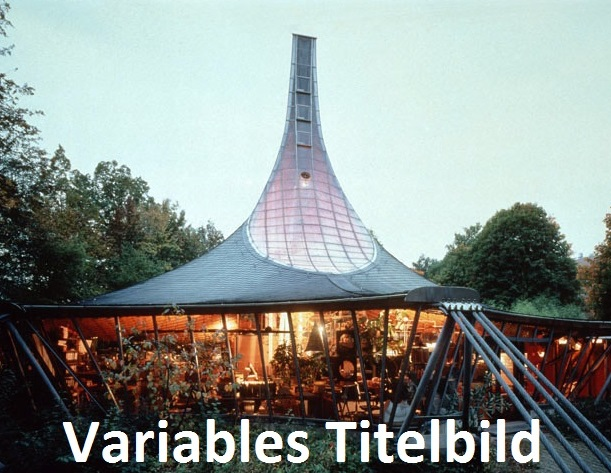
\includegraphics[width=1.0\textwidth]{Titelbild.jpg}
		\end{minipage}
	
	
		\vspace{10mm}
		
		\begin{minipage}[c]{4\baselineskip}
			\vspace{-1mm}
			
\includegraphics[height=3.5\baselineskip]{unistuttgart_logo_de.jpg}
		\end{minipage}
		\begin{minipage}[c]{90mm}
			\small \textsf{Universität Stuttgart} \\
    		\small \textsf{\Institut} \\
    		\small \textsf{\ProfEins} \\
    		\small \textsf{\ProfZwei} 
		\end{minipage}

	\end{minipage}
	\cleardoublepage
\end{titlepage}
%------------------------------------------------------------


\restoregeometry

% ============= Frontmatter ============= 
\frontmatter

\pagestyle{plain.scrheadings} % Leere Kopf- und Fußzeilen
\pagenumbering{Roman} % Römische Seitenzahlen verwenden

\chapter*{Eidesstattliche Erklärung}
% Falls Kapitel nicht im Inhaltsverzeichnis erscheinen soll, folgende Zeile auskommentieren
\addcontentsline{toc}{chapter}{Eidesstattliche Erklärung}
\label{erklaerung}
Hiermit erkläre ich, dass ich die vorliegende Arbeit selbständig verfasst habe, dass ich keine anderen als die angegebenen Quellen benutzt und alle wörtlich oder sinngemäß aus anderen Werken übernommenen Aussagen als solche gekennzeichnet habe, dass die eingereichte Arbeit weder vollständig noch in wesentlichen Teilen Gegenstand eines anderen Prüfungsverfahrens gewesen ist, dass ich die Arbeit weder vollständig noch in Teilen bereits veröffentlicht habe und dass das elektronische Exemplar mit den anderen Exemplaren übereinstimmt. \\
\\[1.5cm]
Datum:	\hrulefill\enspace Unterschrift: \hrulefill
\\[3.5cm]

\vfill

Bitte zitieren Sie diese Arbeit unter Verwendung des folgenden RIS-Eintrages:

\texttt{TY  - THES \\
TI  - \TitelDerArbeit \\
AU  - \StudentNachname, \StudentVorname \\
CN  - \NummerDerArbeit/\StrRight{\EndeJahr}{2} \\
DA  - \Abgabedatum \\
PY  - \EndeJahr \\
M3  - \TypDerArbeit \\
CY  - Stuttgart \\
PB  - Institut für Leichtbau Entwerfen und Konstruieren \\
N1  - \Betreuer
}

\chapter*{Danksagung}
% Falls Kapitel nicht im Inhaltsverzeichnis erscheinen soll, folgende Zeile auskommentieren
\addcontentsline{toc}{chapter}{Danksagung}

\blindtext

\blindtext
% Falls Kapitel nicht im Inhaltsverzeichnis erscheinen soll, folgende Zeile auskommentieren
\addcontentsline{toc}{chapter}{Aufgabenstellung}
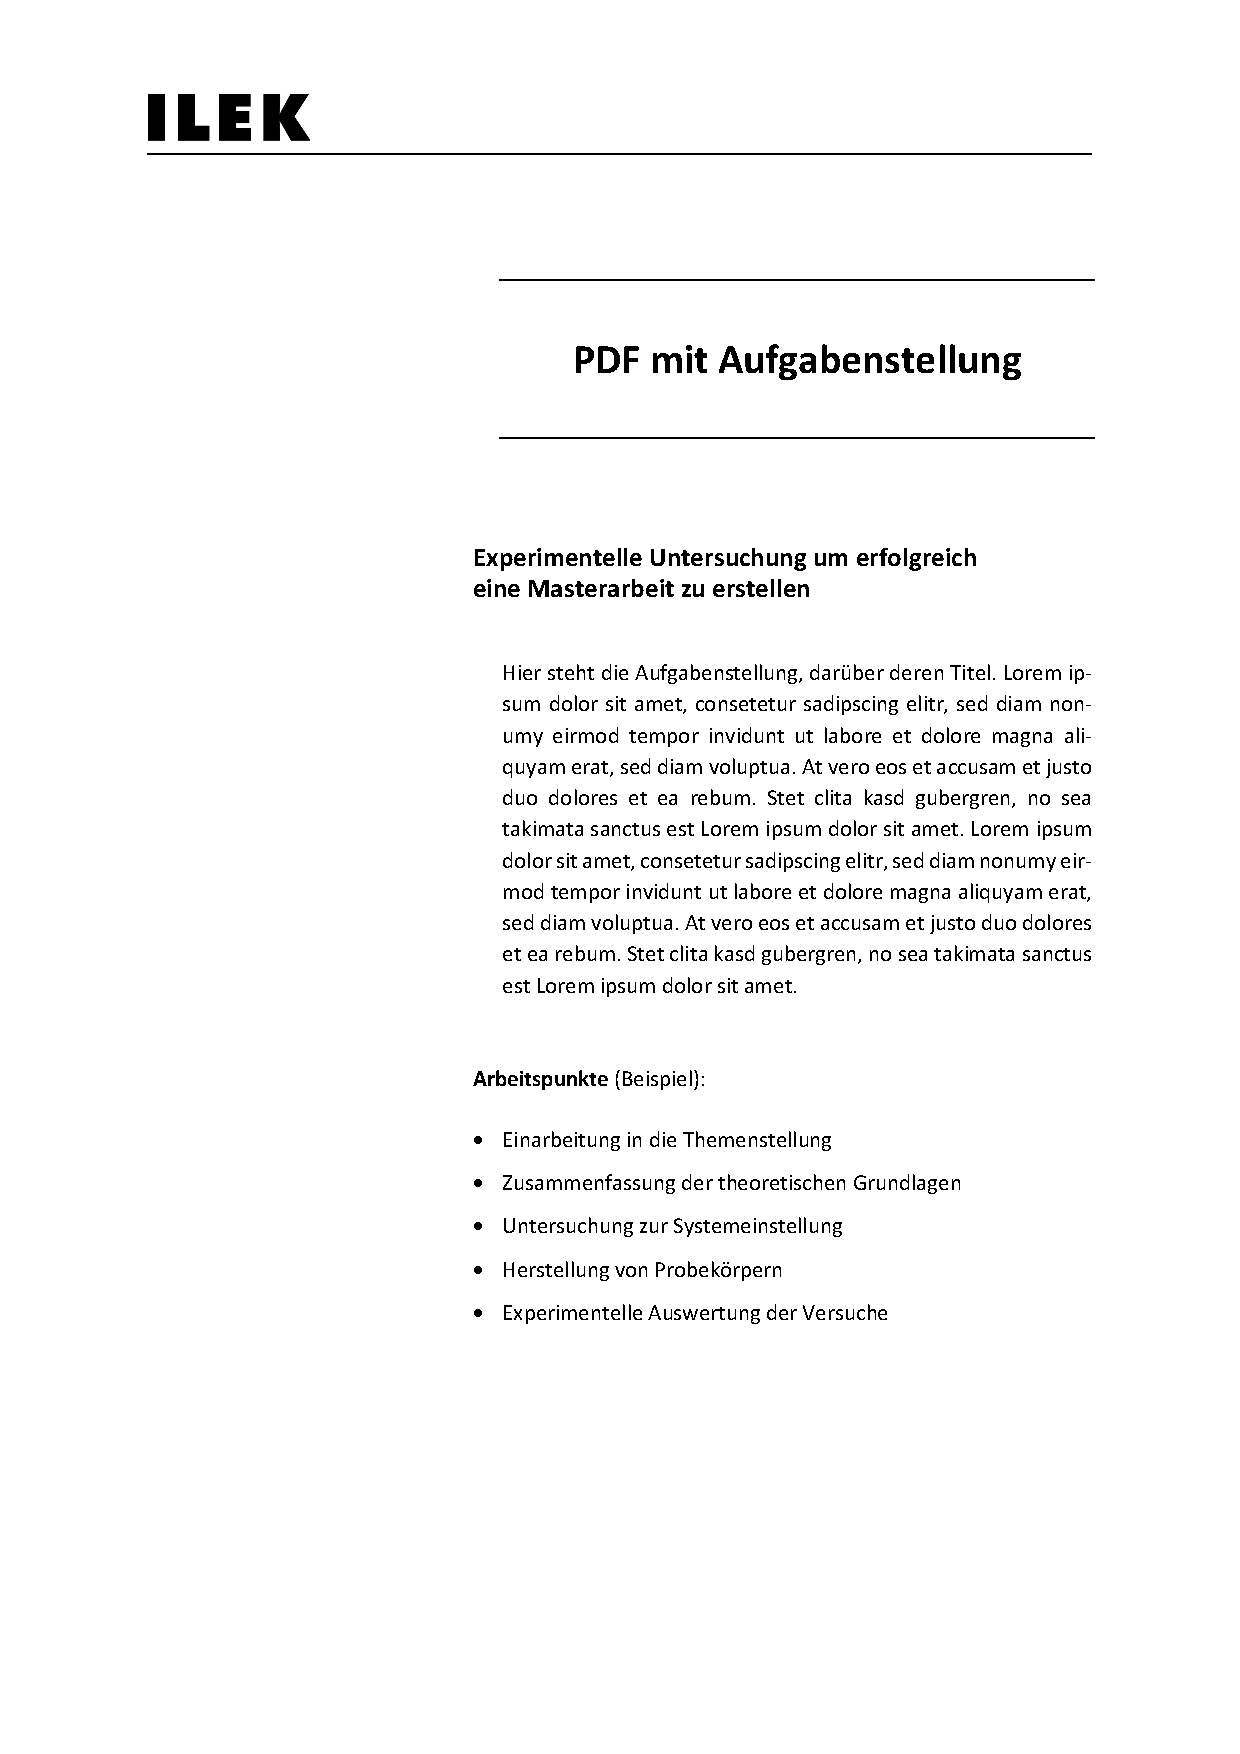
\includepdf[pages=-]{_A_frontmatter/05_assignment/aufgabenstellung.pdf}
\chapter*{Kurzfassung}
% Falls Kapitel nicht im Inhaltsverzeichnis erscheinen soll, folgende Zeile auskommentieren
\addcontentsline{toc}{chapter}{Kurzfassung}

\blindtext

\blindtext

\chapter*{Abstract}
\blindtext

\blindtext

\if 0\autonomenclature
	\chapter*{Nomenklatur}
\addcontentsline{toc}{chapter}{Nomenklatur}
\begin{longtable}{
		@{}
		>{\centering}p{0.15\linewidth}
		@{}
		>{\hspace*{0pt}}p{0.845\linewidth}
		@{}
	}
	\centering
	\small
	\tabularnewline
	\multicolumn{2}{@{}l}{\textsf{\textbf{Akronyme und Abkürzungen}}} \\
	APDL & Ansys Parametric Design Language \\
	DMS & Dehnungsmessstreifen \\
	FEM & Finite-Elemente-Methode \\
	
	\tabularnewline
	\multicolumn{2}{@{}l}{\textsf{\textbf{Lateinische Buchstaben}}} \\
	\textit{a} & Erster Eintrag \\
	\textit{b} & Zweiter Eintrag \\
	
	\tabularnewline
	\multicolumn{2}{@{}l}{\textsf{\textbf{Griechische Buchstaben}}} \\
	$\alpha$ & Kontinuierlicher Temperaturabminderungsfaktor \\
	$\varepsilon$ & Dehnung \\
	$\varepsilon_\mathrm{b}$ & Rechnerische Dehnung im Vierpunktbiegeversuch \\
	
	\tabularnewline
	\multicolumn{2}{@{}l}{\textsf{\textbf{Indizes}}} \\
	aktiv & Wert im aktiven Zustand \\
	min & Minimalwert \\
	
\end{longtable}
\else
	\cleardoublepage

\chapter{Nomenklatur}

% ============= Abkürzungen ============= 

\setglossarysection{section}% <- added					% Titel Abkürzungsverzeichnis auf Ebene "section"
\printacronyms[title=Abkürzungen,style=abbreviation] 	% Abkürzungsverzeichnis hinzufügen

% ============= Symbole ============= 
\addsec[Symbole]{Symbole}

\setglossarysection{subsection}% <- added				% Titel einzelnen Gruppen auf Ebene "subsection"
\glstocfalse											% Folgenden Abschnitte nicht ins TOC

% lat. Großbuchstaben
% Alle Elemente dem Glossary hinzufügen
\glsaddall[types=lat_upp]	
% Vertikalen Abstand vor Titel entfernen
\vspace*{-3em}
% Symbole hinzufügen
\printglossary[title=Lateinische Großbuchstaben,type=lat_upp,nonumberlist,style=symbols]	

% lat. Kleinbuchstaben
\glsaddall[types=lat_low]
\vspace*{-3em}
\printglossary[title=Lateinische Kleinbuchstaben,type=lat_low,nonumberlist,style=symbols]

% gr. Großbuchstaben
\glsaddall[types=gre_upp]
\vspace*{-3em}
\printglossary[title=Griechische Großbuchstaben, type=gre_upp,nonumberlist,style=symbols]

% gr. Kleinbuchstaben
\glsaddall[types=gre_low]
\vspace*{-3em}
\printglossary[title=Griechische Kleinbuchstaben, type=gre_low,nonumberlist,style=symbols]

% mathematische Operatoren
\glsaddall[types=math_op]
\vspace*{-3em}
\printglossary[title=Mathematische Operatoren, type=math_op,nonumberlist,style=symbols]
\fi


\setcounter{tocdepth}{1}    % Inhaltsverzeichnis bis Ebene "Sections"
\tableofcontents            % Inhaltsverzeichnis
\cleardoubleoddpage         % Beginn auf einer neuen Seite. Bei Doppelseiten rechts

% ============= Mainmatter =============
\mainmatter 

\pagestyle{scrheadings}	% pagestyle für gesamtes Dokument aktivieren (Kopf- und Fußzeilen)
\pagenumbering{arabic}	% Arabische Seitenzahlen verwenden

% In diesem Pfad werden die Grafiken geladen
% Dem Pfad für die Grafiken kann durch weitere Einträge in {} ergänzt werden. Default ist nafolgend auskommentiert aufgeführt.
%\graphicspath{{./_E_ressources/images}{./_B_mainmatter/images/}{./_C_appendix/images/}} %Bilderordner

% Hier eigene Kapitel einsetzen
<<<<<<< HEAD
\chapter*{ReadMe}
\addcontentsline{toc}{chapter}{ReadMe}
\label{ReadMe}

Diese Vorlage dient als grober Leitfaden zu Erstellung der Abschlussarbeit. Die Formatierung ist somit nicht zwingend umzusetzen.

Die Formatierung des Deckblattes sollte, soweit möglich, unverändert bleiben. 

Von der Gliederung der Arbeit kann abgewichen werden, solang dieses sinnig begründbar ist.

\section*{LaTeX Grundlagen}

Um mit LaTeX zu Arbeiten, wird einerseits ein Editor und andererseits eine LaTeX-Distribution benötigt. Der Editor dient hierbei zur Eingabe des LaTeX-Code, die LaTeX-Distribution übersetzt den Code in ein Dokument. 

Beispielsweise kann eine Kombination der folgende Programme verwendet werden:

\vspace{-.5cm}
\begin{flalign*}
&\text{1) MiKTeX:} &&\text{\url{https://miktex.org/download}} &&\text{(LaTeX-Distribution)}&\\
&\text{2) TeXstudio:} &&\text{\url{https://www.texstudio.org/}} &&\text{(Editor)} &\\
\end{flalign*}

Alternativ besteht auch die Möglichkeit Online-Dienste zu benutzen, welche mögliche Schwierigkeiten bei der Einrichtung der oben genannten Lösung umgehen. Diese vereinen Editor und LaTeX-Distribution.

\vspace{-.5cm}
\begin{flalign*}
&\text{1) Overleaf:} &&\text{\url{https://de.overleaf.com/}} &&  && \\
\end{flalign*}

Für eine problemlose Kompilierung des \LaTeX-Dokumentes ist es notwendig, einige Einstellungen in der LaTeX-Distribution zu übernehmen.

\begin{description}
	\item[-] Als Standard Bibliographieprogramm sollte Biber ausgewählt werden
	\item[-] Als Standardcompiler wird LuaLaTeX oder PdfLaTeX empfohlen
\end{description}

\newpage

\section*{Hinweis zur Abgabe}

\subsection*{Gedrucktes Exemplar}

In der Regel sollten insgesamt zwei Exemplare an das ILEK ausgehändigt werden. Für den Druck gelten die folgenden Empfehlungen:

\begin{description}
	\item[-] Dickeres Papier (z.B. 100-120 g/m²)
	\item[-] Softcover mit Kaltleimbindundung
	\item[-] Für den Einband sollte das \nameref{section:_01_frontcover}. verwendet werden 
\end{description}

Die Auswahl eines ein- oder doppelseitigen Druckes richtet sich nach der Seitenzahl. Bis ca. 50 Seiten wird ein einseitiger Druck empfohlen, darüber hinaus ein doppelseitiger.

Wichtig bei der Auswahl eines ein- oder doppelseitigen Druckes ist das LaTeX-Dokument entsprechend anzupassen. Dadurch werden die Seitenränder und Seitenzahl korrekt ausgerichtet.

\begin{description}
	\item[-] Doppelseitiger Druck: In der main.tex-Datei die Option \lstinline[basicstyle=\ttfamily]|twoside| auswählen
	\item[-] Einseitiger Druck: In der main.tex-Datei die Option \lstinline[basicstyle=\ttfamily]|twoside| auskommentieren (Standarteinstellung)
\end{description}

Mit diesen Informationen einfach an das Kopiergeschäft herantreten, diese wissen meist was zu tun ist.

\subsection*{Digitales Exemplar (PDF)}

Hierfür in der main.tex-Datei die Option \lstinline[basicstyle=\ttfamily]|twoside| auskommentieren (Standarteinstellung).

Bitte die Arbeit in digitaler Form auf einer CD speichern und einem der gedruckten Exemplare beilegen. Die CD sollte ebenso das LaTeX-Dokument, alle Abbildung und die während der Arbeit erstellten Berechnungen (bswp. in Form von Excel-Tabellen, Programmcode oder FE-Berechnungen ohne Ergebnisse) enthalten.

\newpage

\section*{Aufbau des Ordners}

Der Aufbau des Ordners ist an der Struktur der Abschlussarbeit orientiert. 

Die Ordner und Dateien in denen nicht zwingend Anpassungen vorgenommen werden müssen sind im folgenden gekennzeichnet. Natürlich können diese dennoch angepasst werden.

Hinweise zu den jeweiligen Abschnitten und dem dazugehörigen LaTeX-Code sind auch in den Kommentaren im Code zu finden!\\ 
\\

\dirtree{%
%  .1 JahrNachnameTitelDerArbeit.tex.
 .1 /.
 .2 Jahr\_Nachname\_Titel\_der\_Arbeit.tex.
 .2 Frontcover.tex.
 .2 \_A\_frontmatter.
     .3 01\_frontcover.
     .3 02\_cover.
     .3 03\_copyright.
     .3 04\_acknowledgements.
     .3 05\_assignment.
     .3 06\_abstract.
     .3 07\_nomenclature.
 .2 \_B\_mainmatter.
     .3 examples.tex.
     .3 images.
 .2 \_C\_appendix.
     .3 examples.tex.
     .3 images.
 .2 \_D\_backmatter.
     .3 references.tex.
     .3 literatur.bib.
 .2 \_E\_ressources.
     .3 preambel.tex.
     .3 variables.tex.
     .3 fonts.
     .3 tikz.
}

\section*{JahrNachnameTitelDerArbeit.tex}

Diese Datei ist der Startpunkt des Dokumentes. Hier werden alle im folgenden aufgelisteten Abschnitte referenziert. Um das Gesamtdokument zu erstellen muss diese Datei kompiliert werden.

\section*{Frontcover.tex}

Referenziert auf den Einband der Arbeit. Um den Einband zu erstellen muss diese Datei kompiliert werden.

\newpage

\section*{frontmatter}

Die Titelei (englisch front matter) bezeichnet die Seiten, die dem eigentlichen Inhalt vorangestellt sind.

\subsection*{frontcover}
\label{section:_01_frontcover}

Enthält den Einband der Arbeit. Keine Anpassungen notwendig.

Wichtig: Die Datei Frontcover.pdf dient enthält den Umschlag zur Einreichung beim Druck der Arbeit im Kopiergeschäft. Am besten im Vorraus mit dem Kopiergeschäft abstimmen wie dick die Arbeit wird, sodass der Rücken des Umschlages die richtige Breite hat. Diese hängt ab von der Anzahl der Seiten, der Dicke des Papiers sowie ob ein- oder doppelseitig gedruckt wird. 

Die Breite des Einbandes wird in \nameref{section:_E_ressources_variables} eingestellt.

\subsection*{cover}

Enthält das Titelblatt der Arbeit. 

\subsection*{copyright}

Enthält die eidesstattliche Erklärung zur eigenen Anfertigung der Arbeit. Keine Anpassungen notwendig.

\subsection*{acknowledgements}

Enthält die Danksagung. 

\subsection*{assignment}

Kann optional auch weggelassen werden. Enthält ein PDF mit der Aufgabenstellung.

\subsection*{abstract}

Enthält die englische und deutsche Kurzfassung der Arbeit.

\subsection*{nomenclature}

Enthält Symbole und Abkürzungen die in der Arbeit verwendet werden. Keine Anpassungen notwendig.

Alternativ kann dieser Abschnitt auch ins Backmatter vor das Abbildungsverzeichnis eingefügt werden.

\section*{mainmatter}
\label{section:_A_mainmatter}

Ab hier beginnt der Hauptteil der Abschlussarbeit. Der Aufbau dieses Ordner kann beliebig angepasst werden.

\subsection*{examples.tex}

Die einzelnen Dateien enthalten Beispiele für Formatierungen von Tabellen, Bildern etc. und dienen als Orientierung.

\subsection*{images}

Die verwendeten Abbildungen können in diesem Ordner abgelegt werden. Auch der Aufbau dieses Ordner kann beliebig angepasst werden.

\section*{appendix}

Ab hier beginnt der Anhang der Abschlussarbeit. Auch hier gilt das der Aufbau dieses Ordner beliebig angepasst werden kann.

Der Vorschlag für den Aufbau orientiert sich an \nameref{section:_A_mainmatter}.

\section*{backmatter}

Ab hier beginnet der Schlussteil der Arbeit.

\subsection*{references.tex}

Enthält das Abbildungs-, Tabellen- und Literaturverzeichnis. 

\subsection*{literatur.bib}

Enthält die Daten für das Literaturverzeichnis der Arbeit. Keine Anpassungen notwendig.

Empfohlen wird die Verwaltung und Anfertigung des Literaturverzeichnisses mit den folgenden Programmen. Es bietet sich an bereits zu beginn der Abschlussarbeit alle Quellen mit den genannten Programmen zu verwalten

1. Citavi https://www.citavi.com/de

1. Zotero https://www.zotero.org/

\newpage

\section*{ressources}

Enthält notwendige Einstellungen und Dateien für LaTex.

\subsection*{preambel.tex}

In der Präambel werden alle für das gesamte Dokument gültigen Formatierungseinstellungen getroffen sowie zusätzlich benötigte Pakete geladen. Keine Anpassungen notwendig.

\subsection*{variables.tex}
\label{section:_E_ressources_variables}

Enthält alle wichtigen Angaben (Titel, Betreuer, Jahr ..) zur Arbeit. Diese müssen entsprechend angepasst werden sodass Einband und Titelblatt mit den richtigen Informationen erstellt werden.

\subsection*{fonts}
Enthält die Schriftart der Universität Stuttgart. Aufgrund der Lizenzierung der Schrift dürfen wir die dafür notwendigen Dateien nicht über GitHub zu Verfügung stellen. 

Daher entweder den Betreuer der Arbeit nach den entsprechenden Dateien fragen oder alternativ Arial verwenden (automatisch eingestellt wenn die Schriftart Univers for UniS nicht gefunden wird).

Die Schriftarten der Universität Stuttgart müssen wie folgt benannt werden:

\begin{description}
	\item[-] UniversforUniS45LtObl-Rg
	\item[-] UniversforUniS55Rm-Regular
	\item[-] UniversforUniS65Bd-Regular
\end{description}

\subsection*{tikz}
Durch Tikz kompilierte Grafiken. Keine Anpassungen notwendig.
=======
\chapter*{ReadMe}
\addcontentsline{toc}{chapter}{ReadMe}
\label{ReadMe}

Diese Vorlage dient als grober Leitfaden zu Erstellung der Abschlussarbeit. Die Formatierung ist somit nicht zwingend umzusetzen.

Die Formatierung des Deckblattes sollte, soweit möglich, unverändert bleiben. 

Von der Gliederung der Arbeit kann abgewichen werden, solang dieses sinnig begründbar ist.

\section*{LaTeX Grundlagen}

Um mit LaTeX zu Arbeiten, wird einerseits ein Editor und andererseits eine LaTeX-Distribution benötigt. Der Editor dient hierbei zur Eingabe des LaTeX-Code, die LaTeX-Distribution übersetzt den Code in ein Dokument. 

Beispielsweise kann eine Kombination der folgende Programme verwendet werden:

\vspace{-.5cm}
\begin{flalign*}
&\text{1) MiKTeX:} &&\text{\url{https://miktex.org/download}} &&\text{(LaTeX-Distribution)}&\\
&\text{2) TeXstudio:} &&\text{\url{https://www.texstudio.org/}} &&\text{(Editor)} &\\
\end{flalign*}




Alternativ besteht auch die Möglichkeit Online-Dienste zu benutzen, welche mögliche Schwierigkeiten bei der Einrichtung der oben genannten Lösung umgehen. Diese vereinen Editor und LaTeX-Distribution.

\vspace{-.5cm}
\begin{flalign*}
&\text{1) Overleaf:} &&\text{\url{https://de.overleaf.com/}} &&  && \\
\end{flalign*}

\begin{tcolorbox}[width=\linewidth, sharp corners=all, colback=white!95!black]
How to access the premium features of Overleaf:
\begin{enumerate}
    \item If you have no IEEE Collabratec account, create a free account here: \url{https://ieee-collabratec.ieee.org/}
    \item If you have no Overleaf account, create a free account here: \url{https://www.overleaf.com/register}
    \item Follow the instructions to link your Overleaf account with your IEEE Collabratec account to enable premium features in Overleaf: \url{https://www.overleaf.com/blog/278-how-to-use-overleaf-with-ieee-collabratec-your-quick-guide-to-getting-started}
\end{enumerate}
\end{tcolorbox}

\doublespacing
Für eine problemlose Kompilierung des \LaTeX-Dokumentes ist es notwendig, einige Einstellungen in der LaTeX-Distribution zu übernehmen.

\begin{description}
	\item[-] Als Standard Bibliographieprogramm sollte Biber ausgewählt werden
	\item[-] Als Standardcompiler wird LuaLaTeX oder PdfLaTeX empfohlen
\end{description}

\newpage

\section*{Hinweis zur Abgabe}

\subsection*{Gedrucktes Exemplar}

In der Regel sollten insgesamt zwei Exemplare an das ILEK ausgehändigt werden. Für den Druck gelten die folgenden Empfehlungen:

\begin{description}
	\item[-] Dickeres Papier (z.B. 100-120 g/m²)
	\item[-] Softcover mit Kaltleimbindundung
	\item[-] Für den Einband sollte das \nameref{section:_01_frontcover}. verwendet werden 
\end{description}

Die Auswahl eines ein- oder doppelseitigen Druckes richtet sich nach der Seitenzahl. Bis ca. 50 Seiten wird ein einseitiger Druck empfohlen, darüber hinaus ein doppelseitiger.

Wichtig bei der Auswahl eines ein- oder doppelseitigen Druckes ist das LaTeX-Dokument entsprechend anzupassen. Dadurch werden die Seitenränder und Seitenzahl korrekt ausgerichtet.

\begin{description}
	\item[-] Doppelseitiger Druck: In der main.tex-Datei die Option \lstinline[basicstyle=\ttfamily]|twoside| auswählen
	\item[-] Einseitiger Druck: In der main.tex-Datei die Option \lstinline[basicstyle=\ttfamily]|twoside| auskommentieren (Standarteinstellung)
\end{description}

Mit diesen Informationen einfach an das Kopiergeschäft herantreten, diese wissen meist was zu tun ist.

\subsection*{Digitales Exemplar (PDF)}

Hierfür in der main.tex-Datei die Option \lstinline[basicstyle=\ttfamily]|twoside| auskommentieren (Standarteinstellung).

Bitte die Arbeit in digitaler Form auf einer CD speichern und einem der gedruckten Exemplare beilegen. Die CD sollte ebenso das LaTeX-Dokument, alle Abbildung und die während der Arbeit erstellten Berechnungen (bswp. in Form von Excel-Tabellen, Programmcode oder FE-Berechnungen ohne Ergebnisse) enthalten.

\newpage

\section*{Aufbau des Ordners}

Der Aufbau des Ordners ist an der Struktur der Abschlussarbeit orientiert. 

Die Ordner und Dateien in denen nicht zwingend Anpassungen vorgenommen werden müssen sind im folgenden gekennzeichnet. Natürlich können diese dennoch angepasst werden.

Hinweise zu den jeweiligen Abschnitten und dem dazugehörigen LaTeX-Code sind auch in den Kommentaren im Code zu finden!\\ 
\\

\dirtree{%
%  .1 JahrNachnameTitelDerArbeit.tex.
 .1 /.
 .2 Jahr\_Nachname\_Titel\_der\_Arbeit.tex.
 .2 Frontcover.tex.
 .2 \_A\_frontmatter.
     .3 01\_frontcover.
     .3 02\_cover.
     .3 03\_copyright.
     .3 04\_acknowledgements.
     .3 05\_assignment.
     .3 06\_abstract.
     .3 07\_nomenclature.
 .2 \_B\_mainmatter.
     .3 examples.tex.
     .3 images.
 .2 \_C\_appendix.
     .3 examples.tex.
     .3 images.
 .2 \_D\_backmatter.
     .3 references.tex.
     .3 literatur.bib.
 .2 \_E\_ressources.
     .3 preambel.tex.
     .3 variables.tex.
     .3 fonts.
     .3 tikz.
}

\section*{JahrNachnameTitelDerArbeit.tex}

Diese Datei ist der Startpunkt des Dokumentes. Hier werden alle im folgenden aufgelisteten Abschnitte referenziert. Um das Gesamtdokument zu erstellen muss diese Datei kompiliert werden.

\section*{Frontcover.tex}

Referenziert auf den Einband der Arbeit. Um den Einband zu erstellen muss diese Datei kompiliert werden.

\newpage

\section*{frontmatter}

Die Titelei (englisch front matter) bezeichnet die Seiten, die dem eigentlichen Inhalt vorangestellt sind.

\subsection*{frontcover}
\label{section:_01_frontcover}

Enthält den Einband der Arbeit. Keine Anpassungen notwendig.

Wichtig: Die Datei Frontcover.pdf dient enthält den Umschlag zur Einreichung beim Druck der Arbeit im Kopiergeschäft. Am besten im Vorraus mit dem Kopiergeschäft abstimmen wie dick die Arbeit wird, sodass der Rücken des Umschlages die richtige Breite hat. Diese hängt ab von der Anzahl der Seiten, der Dicke des Papiers sowie ob ein- oder doppelseitig gedruckt wird. 

Die Breite des Einbandes wird in \nameref{section:_E_ressources_variables} eingestellt.

\subsection*{cover}

Enthält das Titelblatt der Arbeit. 

\subsection*{copyright}

Enthält die eidesstattliche Erklärung zur eigenen Anfertigung der Arbeit. Keine Anpassungen notwendig.

\subsection*{acknowledgements}

Enthält die Danksagung. 

\subsection*{assignment}

Kann optional auch weggelassen werden. Enthält ein PDF mit der Aufgabenstellung.

\subsection*{abstract}

Enthält die englische und deutsche Kurzfassung der Arbeit.

\subsection*{nomenclature}

Enthält Symbole und Abkürzungen die in der Arbeit verwendet werden. Keine Anpassungen notwendig.

Alternativ kann dieser Abschnitt auch ins Backmatter vor das Abbildungsverzeichnis eingefügt werden.

\section*{mainmatter}
\label{section:_A_mainmatter}

Ab hier beginnt der Hauptteil der Abschlussarbeit. Der Aufbau dieses Ordner kann beliebig angepasst werden.

\subsection*{examples.tex}

Die einzelnen Dateien enthalten Beispiele für Formatierungen von Tabellen, Bildern etc. und dienen als Orientierung.

\subsection*{images}

Die verwendeten Abbildungen können in diesem Ordner abgelegt werden. Auch der Aufbau dieses Ordner kann beliebig angepasst werden.

\section*{appendix}

Ab hier beginnt der Anhang der Abschlussarbeit. Auch hier gilt das der Aufbau dieses Ordner beliebig angepasst werden kann.

Der Vorschlag für den Aufbau orientiert sich an \nameref{section:_A_mainmatter}.

\section*{backmatter}

Ab hier beginnet der Schlussteil der Arbeit.

\subsection*{references.tex}

Enthält das Abbildungs-, Tabellen- und Literaturverzeichnis. 

\subsection*{literatur.bib}

Enthält die Daten für das Literaturverzeichnis der Arbeit. Keine Anpassungen notwendig.

Empfohlen wird die Verwaltung und Anfertigung des Literaturverzeichnisses mit den folgenden Programmen. Es bietet sich an bereits zu beginn der Abschlussarbeit alle Quellen mit den genannten Programmen zu verwalten

1. Citavi https://www.citavi.com/de

1. Zotero https://www.zotero.org/

\newpage

\section*{ressources}

Enthält notwendige Einstellungen und Dateien für LaTex.

\subsection*{preambel.tex}

In der Präambel werden alle für das gesamte Dokument gültigen Formatierungseinstellungen getroffen sowie zusätzlich benötigte Pakete geladen. Keine Anpassungen notwendig.

\subsection*{variables.tex}
\label{section:_E_ressources_variables}

Enthält alle wichtigen Angaben (Titel, Betreuer, Jahr ..) zur Arbeit. Diese müssen entsprechend angepasst werden sodass Einband und Titelblatt mit den richtigen Informationen erstellt werden.

\subsection*{fonts}
Enthält die Schriftart der Universität Stuttgart. Aufgrund der Lizenzierung der Schrift dürfen wir die dafür notwendigen Dateien nicht über GitHub zu Verfügung stellen. 

Daher entweder den Betreuer der Arbeit nach den entsprechenden Dateien fragen oder alternativ Arial verwenden (automatisch eingestellt wenn die Schriftart Univers for UniS nicht gefunden wird).

Die Schriftarten der Universität Stuttgart müssen wie folgt benannt werden:

\begin{description}
	\item[-] UniversforUniS45LtObl-Rg
	\item[-] UniversforUniS55Rm-Regular
	\item[-] UniversforUniS65Bd-Regular
\end{description}

\subsection*{tikz}
Durch Tikz kompilierte Grafiken. Keine Anpassungen notwendig.
>>>>>>> 990a6cad2dab7d5cf5941d83d63e97e6e59cad28
   % Readme
\chapter{Grundlagen}
\label{ch:01_grundlagen}

\section{Was ist \LaTeX}
\label{sec:01_was_ist_latex}

\LaTeX ist ein Layout- und Satzprogramm für wissenschaftliches Arbeiten. Es basiert auf dem Satzprogramm \TeX\, das von Donald Knuth von der Stanford University entwickelt wurde (seine erste Version erschien 1978).

\section{Textformatierung}
\label{sec:01_textformatierung}

Text kann unter anderem \textit{kursiv}, \textbf{fett} oder \underline{unterstrichen} formatiert werden. Mathematische Zeichen und Formeln können durch spezielle Befehle in \LaTeX erzeugt werden, bspw. $\sigma=E\cdot\varepsilon$.

\section{Gliederung}
\label{sec:01_gliederung}

Im wesentlichen wird das Dokument untergliedert in Kapitel (\verb!\chapter{}!), Abschnitte (\verb!\section{}!) und Unterabschnitte (\verb!\subsection{}!). Auch eine weitere Untergliederung ist möglich. Ab der Ebene (\verb!\subsection{}!) werden Abschnitte in dieser Vorlage im Inhaltsverzeichnis aus Gründen der Übersichtlichkeit nicht abgebildet.

\section{Verweise}
\label{sec:01_verweise}

% Prefixes
% ch: 	    chapter
% sec: 	    section
% subsec: 	subsection
% fig: 	    figure
% tab: 	    table
% eq: 	    equation
% lst: 	    code listing
% itm: 	    enumerated list item
% alg: 	    algorithm
% app: 	    appendix subsection 

Auf Kapitel und Abschnitte kann verwiesen werden. Beispielweise beinhaltet \cref{ch:01_grundlagen} die \crefrange{sec:01_was_ist_latex}{sec:01_zitation}.

Neben Kapiteln und Abschnitten kann auf Bilder, Tabellen, Gleichungen etc. verwiesen werden. Diese müssen im \LaTeX-Code mit \verb!\label{<prefix>:<label>}! versehen werden. 
\section{Zitation}
\label{sec:01_zitation}

Zitate können unter anderem wie folgt eingefügt werden:

\begin{itemize}

    \item Indirektes Zitat, eine Quelle: \cite{yang_application_2003}. 
    
    \item Indirektes Zitat, mehrere Quellen \cite{yang_application_2003, kroll_computational_2016}
    
    \item Direktes Zitat: Wie bereits \citet[][p.97]{yang_application_2003} sagte, \enquote{\lipsum[1][1]}
    
    \item \citet[][p.365]{yang_application_2003} stellte fest: \blockquote{\lipsum[1][2]}
    
\end{itemize}      % Grundlagen
\chapter{Einfügen von Tabellen}
\label{chap:tabellen}

\section{Beispieltabelle}

\begin{table}[h]
	\caption{Beispieltabelle}
	\label{tab:Parameter}
	\centering
	\begin{tabularx}{\textwidth}{p{0.32\textwidth}p{0.32\textwidth}p{0.32\textwidth}}
																					\toprule
		Eins                       	     & Zwei    			& Drei 				\\ 	\midrule
		Vier                       	     & Fünf    			& Sechs				\\
		Sieben                           & Acht         	& Neun				\\ 	\bottomrule	
	\end{tabularx}
\end{table}

\begin{longtabu} to \textwidth {@{} X X[c] X[r] @{}}
	\caption{Tabelle auf Textbreite mit drei gleich großen Spalten}\label{tab:bsp1} \\
	\toprule
	Spalte 1 linksbündig & Spalte 2 zentriert & Spalte 3 rechtsbündig \\
	\midrule
1 , 2                           & 3 , 2                           & 1 , 3 \\
2 , 4                           & 6 , 4                           & 2 , 6 \\
3 , 6                           & 9 , 6                           & 3 , 9 \\
	\bottomrule
\end{longtabu}

\begin{longtabu} to 140mm {@{} X X[c] X[r] @{}}
	\caption{Tabelle auf Textbreite mit drei gleich großen Spalten}\label{tab:bsp2} \\
	\toprule
	Spalte 1 linksbündig & Spalte 2 zentriert & Spalte 3 rechtsbündig \\
	\midrule
1 , 2                           & 3 , 2                           & 1 , 3 \\
2 , 4                           & 6 , 4                           & 2 , 6 \\
3 , 6                           & 9 , 6                           & 3 , 9 \\
	\bottomrule
\end{longtabu}
%

\begin{longtabu} to \textwidth {@{} X[1,l] X[1,c] X[1,r] @{}}
	%----- Kopfzeile erste Tabelle ----- %
	\caption{Tabelle über mehrere Seiten}\label{tab:mehrere Seiten} \\
	\toprule
	Spalte 1 linksbündig & Spalte 2 zentriert & Spalte 3 rechtsbündig \\
	\midrule
	\endfirsthead
	%----- Kopfzeile zweite Tabelle ----- %	
	\caption*{\textbf{Fortsetzung:} \cref{tab:mehrere Seiten}} \\
	\toprule
	Spalte 1 linksbündig & Spalte 2 zentriert & Spalte 3 rechtsbündig \\
	\midrule
	\endhead
	%----- Tabellenende erste Tabelle ----- %	
	\bottomrule
	\endfoot
	%----- Tabellenende zweite Tabelle ----- %
	\bottomrule    
	\endlastfoot
	%----- Inhalt der Tabelle Tabelle ----- %	
1 , 2                           & 3 , 2                           & 1 , 3 \\
2 , 4                           & 6 , 4                           & 2 , 6 \\
3 , 6                           & 9 , 6                           & 3 , 9 \\
4 , 8                           & 12 , 8                           & 4 , 12 \\
5 , 10                           & 15 , 10                           & 5 , 15 \\
6 , 12                           & 18 , 12                           & 6 , 18 \\
7 , 14                           & 21 , 14                           & 7 , 21 \\
8 , 16                           & 24 , 16                           & 8 , 24 \\
9 , 18                           & 27 , 18                           & 9 , 27 \\
10 , 20                           & 30 , 20                           & 10 , 30 \\
11 , 22                           & 33 , 22                           & 11 , 33 \\
12 , 24                           & 36 , 24                           & 12 , 36 \\
13 , 26                           & 39 , 26                           & 13 , 39 \\
14 , 28                           & 42 , 28                           & 14 , 42 \\
15 , 30                           & 45 , 30                           & 15 , 45 \\
16 , 32                           & 48 , 32                           & 16 , 48 \\
17 , 34                           & 51 , 34                           & 17 , 51 \\
18 , 36                           & 54 , 36                           & 18 , 54 \\
19 , 38                           & 57 , 38                           & 19 , 57 \\
\end{longtabu}      % Tabellen
\if 1\autonomenclature \chapter{Abbildungen}
\label{sec:tikz}

Bei wissenschaftlichen Arbeiten sollten aussagekräftige Bildunterschriften angefertigt werden. Abbildungen sind meist nicht als selbsterklärend zu verstehen. Daher müssen zusätzliche Beschreibungen in die Bildunterschrift eingefügt werden, die es dem Leser möglichst erlauben, nur durch die Abbildung und dessen Beschreibung die im Fließtext erläuterten Zusammenhänge zusammengefasst zu verstehen oder mindestens die Bedeutung der Abbildung für Teile des Fließtextes klar einordnen zu können.

Zur Erstellung von aufschlussreichen Abbildungen siehe auch das \verb!Graphic-design-cheat-sheet.pdf!

\section{Einfügen von Bildern}
\label{sec:graf}

\subsection{Einfaches Bild}

\begin{figure}[H]
  \centering  
  	
\includegraphics[scale=0.5]{ILEK-logo.jpg}
  \caption{ILEK Logo}
  \label{fig:05_starwars}
\end{figure}

\subsection{Gruppierung von Bildern}

\begin{figure}[H]
	\centering
	\begin{subfigure}[b]{0.3\textwidth}
		\centering
		
\includegraphics[width=\textwidth]{ILEK-logo.jpg}
		\caption{$y=x$}
		\label{fig:05_a}
	\end{subfigure}
%	\hfill
\hspace{1cm}
	\begin{subfigure}[b]{0.3\textwidth}
		\centering
		
\includegraphics[width=\textwidth]{ILEK-logo.jpg}
		\caption{$y=3sinx$}
		\label{fig:05_b}
	\end{subfigure}
	\\ 
	\begin{subfigure}[b]{0.3\textwidth}
		\centering
		
\includegraphics[width=\textwidth]{ILEK-logo.jpg}
		\caption{$y=3sinx$}
		\label{fig:05_c}
	\end{subfigure}
%	\hfill
\hspace{1cm}
	\begin{subfigure}[b]{0.3\textwidth}
		\centering
		
\includegraphics[width=\textwidth]{ILEK-logo.jpg}
		\caption{$y=5/x$}
		\label{fig:05_five over x}
	\end{subfigure}
	\caption{Vier Bilder}
	\label{fig:05_d}
\end{figure}

\newpage

\subsection{Bilder und Tabellen im Fließtext}

\begin{wraptable}[]{o}[0cm]{9cm}
	\begin{center}
		\begin{tabular}{|l|l|l|}
			\hline
			r & R & right side of the text\\
			l & L & left side of the text\\
			i & I & inside edge–near the binding\\
			& &  (in a twoside document)\\
			o & O & outside edge–far from the binding\\
			\hline
		\end{tabular}
	\end{center}
	\caption{The uppercase version allows the figure to float. The lowercase version means exactly here.}%\citep{cite}
\end{wraptable}

\blindtext[2]

%\begin{wrapfigure}[Zeile]{Position}[Randüberhang]{Breite}
\begin{wrapfigure}[]{o}[0cm]{6.5cm}
	
\includegraphics[width=6cm,angle=0]{ILEK-logo.jpg}
	\caption{Bildbezeichnung}
	\label{fig:05_bild}
\end{wrapfigure}

\blindtext[2]

\newpage

\section{Eigene Diagramme/Grafiken}

Es gibt viele Möglichkeiten eigene Diagramme und Grafiken zu erstellen und in das \LaTeX-Dokument einzubinden. Im folgenden werden beispielhaft die Erstellung von \nameref{subsec:python_inkscape} sowie die Erstellung von \nameref{subsec:tikz} erläutert.

\subsection{Diagramme und Grafiken mit Inkscape}
\label{subsec:python_inkscape}

Grafiken und Skizzen können als Vektorgrafik direkt in Inkscape (\url{https://inkscape.org/de/}) erstellt werden.

Diagramme lassen sich mit Hilfe der Programmiersprache Python erstellen. Zu diesem Zweck werden die Daten zunächst mit Python verarbeitet und anschließend bspw. mit Matplotlib (\url{https://matplotlib.org/}), Seaborn (\url{https://seaborn.pydata.org/}) und/oder Plotly (\url{https://plotly.com/}) geplottet.

Empfohlen wird die Plots als \gls{SVG} zu speichern. Diese können dann bei Bedarf in Inkscape nachbearbeitet werden. 

\begin{figure}[ht]
    \begin{footnotesize}
    	\centering
    	\begin{subfigure}[b]{0.45\textwidth}
    		\centering
    		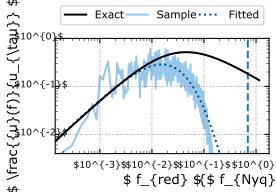
\includegraphics{PSD_Mesh_A_PNG.png}
    		\caption{%
    		    Diagramm direkt als .png importiert. Schriftarten und Schriftgröße werden nicht angepasst, mathematische Symbole können nicht verwendet werden.
    		}
    		\label{fig:png_import}
    	\end{subfigure}
    	\hspace{0.05\textwidth}
    	\begin{subfigure}[b]{0.45\textwidth}
    		\centering
    		\input{_B_mainmatter/images/PSD_Mesh_A.pdf_tex}
    		\caption{%
    		    Diagramm als .svg importiert. Schriftarten und Schriftgröße werden auf das Dokument angepasst und mathematische Symbole werden konvertiert.
    		}
    		\label{fig:svg_import}
    	\end{subfigure}
    \end{footnotesize}
\end{figure}

Es existieren mehrere Möglichkeiten die .svg-Grafiken einzubinden. Siehe \url{https://tex.stackexchange.com/questions/2099/how-to-include-svg-diagrams-in-latex} für eine detaillierte Beschreibung der folgenden beiden Methoden. 

\subsubsection{1) Einbindung als .svg}

Hierfür kann das Paket \href{https://www.ctan.org/tex-archive/graphics/svg}{svg} verwendet werden. Jede SVG-Datei, die mit dem Befehl \verb!\includesvg! übergeben wird, wird unter der Haube mit Hilfe einiger Zusatzprogramme konvertiert.

Leider funktioniert dies nicht immer problemlos, da die Zusatzprogramme meist nicht standardmäßig installiert sind. Ansonsten ist dies aber die zu bevorzugenden Variante.

Prinzipiell kann die \gls{SVG}-Grafik direkt wie folgt eingebunden werden:

\begin{Verbatim}
\begin{figure}
    \input{filename}
\end{figure}
\end{Verbatim}

\newpage

\subsubsection{2) Einbindung als .pdf\_tex}

Die \gls{SVG}-Grafiken müssen in Inkscape als .pdf und .pdf\_tex exportiert werden. Hierzu die \gls{SVG}-Grafik als .pdf speichern und die Option \flqq Text in PDF weglassen und \LaTeX Datei erstellen \frqq auswählen. Dadurch werden Alle Texte aus der .pdf entfernt, in die .pdf\_tex exportiert und werden beim Einbinden in das \LaTeX-Dokument mit den Dokumenteneinstellungen formatiert.

Dieser Schritt kann auch entweder durch die Erstellung eines Batch-Skriptes, dem direkten Export aus o.g. Programmen als .pdf\_tex oder der Programmierung eines Latex-Befehls welcher Inkscape nutzt um den .pdf\_tex Export durchzuführen automatisiert werden, siehe auch \url{https://github.com/BeneStrahm/pyLEK/tree/master/inkscape}.

Anschließend kann die Grafik wie folgt eingebunden werden:

\begin{Verbatim}
\begin{figure}
    \input{filename.pdf_tex}
\end{figure}
\end{Verbatim}

\newpage

\section{Diagramme und Grafiken mit tikz}
\label{subsec:tikz}

\subsubsection{Darstellung von Funktionen}

\begin{figure}[htb]
\centering
\begin{align*}
f(x)=\tanh(x)
\end{align*}
\begin{tikzpicture}
\begin{axis}
[
width=200pt,
height=200pt,
axis x line=middle, xmin=-4, xmax=4, xtick={-3,...,3}, xlabel=$x$,
axis y line=middle, ymin=-1.5, ymax=1.5, ytick={-1,...,1}, ylabel=$f(x)$,
scale only axis=true,
samples=101
]
\addplot[uniSdarkblue, mark=none, very thick]{tanh(x)};
%		\legend{$\tanh(x)$}
\end{axis}
\end{tikzpicture}
\caption[Tangens hyperbolicus Aktivierungsfunktion]{Tangens hyperbolicus}
\label{fig:05_AktivTan}
\end{figure}

\subsubsection{for-Schleifen bei der Grafikerzeugung}

\begin{figure}[htb]
	\centering
	\begin{tikzpicture}[]
	\tikzstyle{netnode}=[circle, inner sep=0pt, text width=22pt, align=center, line width=1.0pt]
	\tikzstyle{inputnode}=[netnode, fill=uniSlightgrey,draw=black]
	\tikzstyle{hiddennode}=[netnode, fill=uniSlightgrey,draw=black]
	\tikzstyle{outputnode}=[netnode, fill=uniSlightgrey,draw=black]
	\tikzstyle{signal}=[arrows={-latex},draw=uniSblack,line width=1pt,rounded corners=4pt]
	
	\def\nodedist{35pt}
	\def\layerdist{80pt}
	\def\pindist{20pt}
	
	\tikzstyle{every pin edge}=[signal]
	\tikzstyle{annot} = [text width=6em, text centered]
	
	\foreach \y in {1,...,3}
	\node[inputnode, pin={[pin edge={latex-}, pin distance=\pindist]left:Eingabe \y}] 
	(I\y) at (0,-\y*\nodedist) {$i_\y$};  
	
	\foreach \y in {1,...,4}
	\node[hiddennode] 
	(H1\y) at ($(\layerdist,-\y*\nodedist) +(0, 0.5*\nodedist)$) {$h_\y^1$};
	
	\foreach \y in {1,...,4}
	\node[hiddennode] 
	(H2\y) at ($(2*\layerdist,-\y*\nodedist) +(0, 0.5*\nodedist)$) {$h_\y^2$};
	
	\foreach \y in {1,...,2}
	\node[outputnode, pin={[pin edge={-latex}, pin distance=\pindist]right:Ausgabe \y}]
	(O\y) at ($(H21) + (\layerdist, -\y*\nodedist)$) {$o_\y$};
	
	\foreach \dest in {1,...,4}
	\foreach \source in {1,...,3}
	\draw[signal] (I\source) -- (H1\dest);
	
	\foreach \dest in {1,...,4}
	\foreach \source in {1,...,4}
	\draw[signal] (H1\source) -- (H2\dest);
	
	\foreach \dest in {1,...,2}
	\foreach \source in {1,...,4}
	\draw[signal] (H2\source) edge (O\dest);
	
	\node[annot, above=4pt of H11] (hl) {verborgene Schicht 1};
	\node[annot, above=4pt of H21] (hl) {verborgene Schicht 2};
	\node[annot] at (I1 |- hl) {Eingabe\-schicht};
	\node[annot] at (O1 |- hl) {Ausgabe\-schicht};
	\end{tikzpicture}
	\caption[Schematischer Aufbau eines künstlichen neuronalen Netzes] %hier kann ein alternativer/ verkürzter Text für das Abbildungsverzeichnis angegeben werden
	{Schematischer Aufbau eines künstlichen neuronalen Netzes \cite[Abb. nach][]{Frochte.2019}} %Bildunteschrift
	\label{fig:05_DNN}
\end{figure}

\newpage

\subsubsection{Einbeziehung von Daten aus CSV-Datei}

\setlength{\figureheight}{5cm}
\setlength{\figurewidth}{\textwidth}
\begin{figure}[htbp]
	\centering
	\begin{tikzpicture}
		\begin{axis}[
			width=\figurewidth,
			height=\figureheight,
			date coordinates in = x,
			xmin=2018-01-01 00:00,
			xmax=2018-01-08 00:00,
			minor x tick num=1,
			xtick={2018-01-01 12:00, 2018-01-02 12:00, 2018-01-03 12:00, 2018-01-04 12:00, 2018-01-05 12:00, 2018-01-06 12:00, 2018-01-07 12:00},
			set layers,cell picture=true,
			xticklabel={\day.\month},
			xlabel={2018},
			ymin=-0.1, ymax=1.1, ytick={0,0.5,1},
			no marks,
			scaled y ticks = false,
			ylabel={[\nicefrac{\%}{100}]}
			,]
			\addplot+[color=black ] table[x=Zeit, y=Shadestep, col sep=comma, skip first n=0] {_B_mainmatter/data/Example.csv};
			\legend{Shadestep};
		\end{axis}
	\end{tikzpicture}
	\caption[Photometrische Regelung der adaptiven Verglasung im Juli 2018, nach 500 Episoden]{Photometrische Regelung der adaptiven Verglasung nach 500 Episoden, für den Zeitraum vom 01. bis 07. Juli 2018} \label{fig:05_AVPhJun500}	
\end{figure}

\ifLuaTeX %PDFLaTeX kommt beim internen Speichermanagement schnell an seine grenzen, weshalb dieser Plot nur beim Kompilieren in LuaLaTeX angezeigt wird.
\subsubsection{Einbeziehung von Daten aus CSV-Datei und Gruppierung von Grafiken}

\begin{figure}[htb]
	\setlength{\figureheight}{5cm}
	\setlength{\figurewidth}{\textwidth}
	\centering
	\begin{tikzpicture}
		\begin{groupplot}[
			width=\figurewidth,
			height=\figureheight,
			date coordinates in = x,
			xmin=2018-01-01 00:00,
			xmax=2018-01-08 00:00,
			minor x tick num=1,
			xtick={2018-01-01 12:00, 2018-01-02 12:00, 2018-01-03 12:00, 2018-01-04 12:00, 2018-01-05 12:00, 2018-01-06 12:00, 2018-01-07 12:00},
			set layers,cell picture=true,
			xticklabel={\day.\month},
			xlabel={2018},
			no marks,
			scaled y ticks = false,
			group style = {group size = 1 by 7,
				horizontal sep =1cm,
				vertical sep = 0cm,},]
			
			\nextgroupplot[xlabel={},xticklabels={},ylabel={[°C]}]
			\addplot[color=black ] table[x=Zeit, y=T01, col sep=comma, skip first n=0] {_B_mainmatter/data/Example.csv};
			\legend{T01};
			
			\nextgroupplot[xlabel={},xticklabels={},ylabel={[klx]}]
			\addplot[color=black ] table[x=Zeit, y expr=\thisrow{B01}/1000, col sep=comma, skip first n=0] {_B_mainmatter/data/Example.csv};
			\legend{B01};
			
			\nextgroupplot[ylabel={[kW]}, ymin=-0.02, ymax=0.32, ytick={0,0.1,0.2,0.3},]
			\addplot+[color=black , name path=A] table[x=Zeit, y expr=\thisrow{QBeleuchtung}+\thisrow{QHeizung}+\thisrow{QKuehlung}, col sep=comma, skip first n=0] {_B_mainmatter/data/Example.csv};
			\addplot+[draw=none,name path=B, mark=none] table[x=Zeit, y expr=0, col sep=comma, skip first n=0] {_B_mainmatter/data/Example.csv}; 
			\addplot+[gray, fill opacity=0.1] fill between[of=A and B];
			\legend{Q\textsubscript{HEAT}+Q\textsubscript{COOL}+Q\textsubscript{LIGHT}};

		\end{groupplot}
	\end{tikzpicture}
	\caption[Kombinierte Regelung im Januar 2018, nach 500 Episoden]{Kombinierte Regelung nach 500 Episoden, für den Zeitraum vom 01. bis 07. Januar 2018} \label{fig:05_KomJan18}	
\end{figure}
\fi \fi  % Abbildungen
\chapter{Mathematische Beispiele}
\label{sec:math}

\section{Gleichungen}

\begin{align}
\sin A \cos B &= \frac{1}{2}\left[ \sin(A-B)+\sin(A+B) \right] \\
\sin A \sin B &= \frac{1}{2}\left[ \sin(A-B)-\cos(A+B) \right] \\
\cos A \cos B &= \frac{1}{2}\left[ \cos(A-B)+\cos(A+B) \right] 
\end{align}

\begin{align*}
\sin A \cos B &= \frac{1}{2}\left[ \sin(A-B)+\sin(A+B) \right] \\
\sin A \sin B &= \frac{1}{2}\left[ \sin(A-B)-\cos(A+B) \right] \\
\cos A \cos B &= \frac{1}{2}\left[ \cos(A-B)+\cos(A+B) \right] 
\end{align*}

\[
\int_a^bu\frac{d^2v}{dx^2}\,dx
=\left.u\frac{dv}{dx}\right|_a^b
-\int_a^b\frac{du}{dx}\frac{dv}{dx}\,dx.
\]

\section{Arrays}

\[
\begin{bmatrix}
1 & x & 0 \\
0 & 1 & -1
\end{bmatrix}\begin{bmatrix}
1  \\
y  \\
1
\end{bmatrix}
=\begin{bmatrix}
1+xy  \\
y-1
\end{bmatrix}.
\]


\[
|x|=\begin{cases}
x, & \text{if }x\geq 0\,,  \\
-x, & \text{if }x< 0\,.
\end{cases}
\]


\[
\begin{matrix}
-2 & 1 & 0 & 0 & \cdots & 0  \\
1 & -2 & 1 & 0 & \cdots & 0  \\
0 & 1 & -2 & 1 & \cdots & 0  \\
0 & 0 & 1 & -2 & \ddots & \vdots \\
\vdots & \vdots & \vdots & \ddots & \ddots & 1  \\
0 & 0 & 0 & \cdots & 1 & -2
\end{matrix}
\]      % Formeln
\if 1\autonomenclature \chapter{Nomenklatur}

Die Nomenklatur ist gegliedert in Abkürzungen und Symbole. Die Symbole sind gegliedert in lateinische sowie griechische Klein- und Großbuchstaben. Jeder dieser Teile hat ein eigenes Glossar in LaTeX. 

Diese Gliederung dient als Richtlinie. Wird eine andere Gliederung verwendet, müssen die Preambel und die Dateien unter \lstinline[basicstyle=\ttfamily]|_A_frontmatter\07_nomenclature| angepasst werden

\section{Abkürzungen}
Abkürzungen müssen unter \lstinline[basicstyle=\ttfamily]|_A_frontmatter\07_nomenclature\_abbreviations.tex| definiert werden. Sie erscheinen nur im Abkürzungsverzeichnis insofern sie im Dokument verwendet werden. 

Bei erstmaliger Verwendung, bspw. \gls{CFD} wird automatisch die Langform im Fließtext verwendet. Für die nachfolgende Verwendung wird die Kurzform, bspw. \gls{CFD} verwendet.

Verwendet werden in diesem Beispiel die Abkürzungen \gls{cent}, \gls{DFT}, \gls{FEM},  sowie \gls{FV}.

\section{Symbole}

Abkürzungen müssen unter \lstinline[basicstyle=\ttfamily]|_A_frontmatter\07_nomenclature\_symbols.tex| definiert werden. Standartmäßig erscheinen alle Symbole in der Nomenklatur, auch wenn Sie nicht im Dokument verwendet werden. 

Gegliedert sind die Symbole in:

Lateinische Kleinbuchstaben, bspw. \gls{u_i}, \gls{u_ref}

Lateinische Großbuchstaben, bspw. \gls{Strouhal}, \gls{Iuu}

Griechische Kleinbuchstaben, bspw. \gls{kappa}, \gls{rho}

Griechische Großbuchstaben, bspw. \gls{dt}

Mathematische Operatoren, bspw. \gls{mean}, \gls{std} 

\newpage

\section{Hinweise zum Kompilieren}

Wird das Dokument, z.B. eines mit dem Namen "main.tex", auf dem lokalen Rechner kompiliert, folgende Reihenfolge  verwenden:

Bspw. mit pdflatex als Compilier:

pdflatex main.tex

makeglossaries glossaries

pdflatex main.tex

Um in Overleaf zu kompilieren, müssen diese Schritte nicht beachtet werden. Allerdings gibt es hier teilweise Probleme. Sollte etwas nicht korrekt funktionieren, lohnt es sich für die Erstellung der Nomenklatur den Compiler zu wechseln und den Cache zu leeren. Siehe auch Online die Hinweise von Overleaf zum Thema "Glossaries". \fi   % Nomenklatur
\chapter{Erweiterte Formatierung}

\section{Float Objekte}

\begin{description}
	\item[h:] an der Stelle, an der es in der Eingabedatei angegeben ist (here)
	\item[t:] am oberen Ende der aktuellen oder Folgeseite (top)
	\item[b:] am unteren Ende der aktuellen Seite (bottom)
	\item[p:] auf einer eigenen Seite für ein oder mehrere Gleitobjekte (page)
	\item[!:] Überschreiben Sie die internen Parameter, die LaTeX zur Bestimmung "guter" Gleitkommapositionen verwendet.
	\item[H:] Setzt den Float an genau die Stelle im LaTeX-Code. Erfordert das float-Paket.
\end{description}

\section{Einheiten}
Bei der Verwendung von Einheiten wird in der Regel bei Wissenschaftlichen Arbeiten ein schmales Leerzeichen verwendet.\\
1 m : Leerzeichen \\
1\,m : schmales Leerzeichen \\      % Erweiterte Formatierung
\chapter{Farbschema}

Es sollen möglichst die folgenden Farben für eigens erstelle Diagramme und Abbildungen verwendet werden, dabei kann zwischen einem farbigen Schema oder Graustufen gewählt werden.

\subsubsection{Uni Stuttgart farbig}
\begin{testcolors}[RGB,HTML]
    \testcolor{uniSlightblue}
    \testcolor{uniSdarkblue}
    \testcolor{uniSdarkgrey}
    \testcolor{uniSgreyblue}
    \testcolor{uniSgrey}
\end{testcolors}

\subsubsection{Uni Stuttgart Graustufen}
\begin{testcolors}[RGB,HTML]
    \testcolor{uniSblack}
    \testcolor{uniSdarkgrey}
    \testcolor{uniSgrey}
    \testcolor{uniSlightgrey}
\end{testcolors}      % Farbschema
\chapter{Einfügen von Quellcode}
\label{chap:code}

\section{Beispiel für einen Programmcode}


\if 1\mintedinstall
\subsection{Beispiel Minted}
	\begin{minted}[xleftmargin=20pt,linenos]{python}
	import numpy as np
	
	def incmatrix(genl1,genl2):
		m = len(genl1)
		n = len(genl2)
		M = None #to become the incidence matrix
		VT = np.zeros((n*m,1), int)  #dummy variable
	
		#compute the bitwise xor matrix
		M1 = bitxormatrix(genl1)
		M2 = np.triu(bitxormatrix(genl2),1) 
	
		for i in range(m-1):
			for j in range(i+1, m):
				[r,c] = np.where(M2 == M1[i,j])
				for k in range(len(r)):
					VT[(i)*n + r[k]] = 1;
					VT[(i)*n + c[k]] = 1;
					VT[(j)*n + r[k]] = 1;
					VT[(j)*n + c[k]] = 1;
					
					if M is None:
						M = np.copy(VT)
					else:
						M = np.concatenate((M, VT), 1)
					
					VT = np.zeros((n*m,1), int)
	
		return M
	\end{minted}
\fi




\subsection{Beispiel listings}
\begin{lstlisting}[language=Python]
import numpy as np

def incmatrix(genl1,genl2):
	m = len(genl1)
	n = len(genl2)
	M = None #to become the incidence matrix
	VT = np.zeros((n*m,1), int)  #dummy variable

	#compute the bitwise xor matrix
	M1 = bitxormatrix(genl1)
	M2 = np.triu(bitxormatrix(genl2),1) 
	
	for i in range(m-1):
		for j in range(i+1, m):
			[r,c] = np.where(M2 == M1[i,j])
			for k in range(len(r)):
				VT[(i)*n + r[k]] = 1;
				VT[(i)*n + c[k]] = 1;
				VT[(j)*n + r[k]] = 1;
				VT[(j)*n + c[k]] = 1;
	
				if M is None:
					M = np.copy(VT)
				else:
					M = np.concatenate((M, VT), 1)
				
				VT = np.zeros((n*m,1), int)
				
	return M
\end{lstlisting}

      % Programmcode

% ============= Appendix =============
\appendix

\addappheadtotoc
\appendixpage

\chapter{Exemplarischer Anhang}
\label{chap:tab}

\section{Beispieltabelle}

\begin{table}[h]
	\caption{Beispieltabelle}
	\label{tab:par}
	\centering
	\begin{tabularx}{\textwidth}{p{0.32\textwidth}p{0.32\textwidth}p{0.32\textwidth}}
																					\toprule
		Eins                       	     & Zwei    			& Drei 				\\ 	\midrule
		Vier                       	     & Fünf    			& Sechs				\\
		Sieben                           & Acht         	& Neun				\\ 	\bottomrule	
	\end{tabularx}
\end{table}

\begin{longtabu} to \textwidth {@{} X X[c] X[r] @{}}
	\caption{Tabelle auf Textbreite mit drei gleich großen Spalten} \\
	\toprule
	Spalte 1 linksbündig & Spalte 2 zentriert & Spalte 3 rechtsbündig \\
	\midrule
1 , 2                           & 3 , 2                           & 1 , 3 \\
2 , 4                           & 6 , 4                           & 2 , 6 \\
3 , 6                           & 9 , 6                           & 3 , 9 \\
	\bottomrule
\end{longtabu}

\begin{longtabu} to 140mm {@{} X X[c] X[r] @{}}
	\caption{Tabelle auf Textbreite mit drei gleich großen Spalten} \\
	\toprule
	Spalte 1 linksbündig & Spalte 2 zentriert & Spalte 3 rechtsbündig \\
	\midrule
1 , 2                           & 3 , 2                           & 1 , 3 \\
2 , 4                           & 6 , 4                           & 2 , 6 \\
3 , 6                           & 9 , 6                           & 3 , 9 \\
	\bottomrule
\end{longtabu}

\begin{longtabu} to \textwidth {@{} X[1,l] X[1,c] X[1,r] @{}}
	%----- Kopfzeile erste Tabelle ----- %
	\caption{Tabelle über mehrere Seiten}\label{tab:mehrere Seiten Anhang} \\
	\toprule
	Spalte 1 linksbündig & Spalte 2 zentriert & Spalte 3 rechtsbündig \\
	\midrule
	\endfirsthead
	%----- Kopfzeile zweite Tabelle ----- %	
	\caption*{\textbf{Fortsetzung:} \Cref{tab:mehrere Seiten Anhang}} \\
	\toprule
	Spalte 1 linksbündig & Spalte 2 zentriert & Spalte 3 rechtsbündig \\
	\midrule
	\endhead
	%----- Tabellenende erste Tabelle ----- %	
	\bottomrule
	\endfoot
	%----- Tabellenende zweite Tabelle ----- %
	\bottomrule    
	\endlastfoot
	%----- Inhalt der Tabelle Tabelle ----- %	
	1 , 2                           & 3 , 2                           & 1 , 3 \\
	2 , 4                           & 6 , 4                           & 2 , 6 \\
	3 , 6                           & 9 , 6                           & 3 , 9 \\
	4 , 8                           & 12 , 8                           & 4 , 12 \\
	5 , 10                           & 15 , 10                           & 5 , 15 \\
	6 , 12                           & 18 , 12                           & 6 , 18 \\
	7 , 14                           & 21 , 14                           & 7 , 21 \\
	8 , 16                           & 24 , 16                           & 8 , 24 \\
	9 , 18                           & 27 , 18                           & 9 , 27 \\
	10 , 20                           & 30 , 20                           & 10 , 30 \\
	11 , 22                           & 33 , 22                           & 11 , 33 \\
	12 , 24                           & 36 , 24                           & 12 , 36 \\
	13 , 26                           & 39 , 26                           & 13 , 39 \\
	14 , 28                           & 42 , 28                           & 14 , 42 \\
	15 , 30                           & 45 , 30                           & 15 , 45 \\
	16 , 32                           & 48 , 32                           & 16 , 48 \\
	17 , 34                           & 51 , 34                           & 17 , 51 \\
	18 , 36                           & 54 , 36                           & 18 , 54 \\
	19 , 38                           & 57 , 38                           & 19 , 57 \\
\end{longtabu}


% ============= Backmatter =============
\backmatter

%Literaturverzeichnis
\printbibliography[title=Literaturverzeichnis] 

%Verzeichnis aller Bilder
\listoffigures 

%Verzeichnis aller Tabellen
\listoftables 

\end{document}